\chapter*{Test a guitars frequency area}
A test was made to get a view of the frequency area, in which the tones from a guitar lies.

\section*{Materials and setup}
To measure the frequency area on a guitar, the following materials are used:
\begin{itemize}
\item Digilent Analog Discovery 2 (Oscilloscope)
\item Fender Squier Classic Vibe Telecaster (Guitar)
\item Digilent Waveforms 2015 (PC - software)
\end{itemize}

\begin{figure}[htbp!]
\centering
\def\svgwidth{\columnwidth}
\chapter{Test a guitars frequency area}\label{app:frequency_area}
A test was made to get a view of the frequency area, in which the tones from a guitar lies.

\section*{Materials and setup}
To measure the frequency area on a guitar, the following materials are used:
\begin{itemize}
\item Digilent Analog Discovery 2 (Oscilloscope)
\item Fender Squier Classic Vibe Telecaster (Guitar)
\item Digilent Waveforms 2015 (PC - software)
\end{itemize}

\begin{figure}[htbp!]
\centering
\def\svgwidth{\columnwidth}
\chapter{Test a guitars frequency area}\label{app:frequency_area}
A test was made to get a view of the frequency area, in which the tones from a guitar lies.

\section*{Materials and setup}
To measure the frequency area on a guitar, the following materials are used:
\begin{itemize}
\item Digilent Analog Discovery 2 (Oscilloscope)
\item Fender Squier Classic Vibe Telecaster (Guitar)
\item Digilent Waveforms 2015 (PC - software)
\end{itemize}

\begin{figure}[htbp!]
\centering
\def\svgwidth{\columnwidth}
\chapter{Test a guitars frequency area}\label{app:frequency_area}
A test was made to get a view of the frequency area, in which the tones from a guitar lies.

\section*{Materials and setup}
To measure the frequency area on a guitar, the following materials are used:
\begin{itemize}
\item Digilent Analog Discovery 2 (Oscilloscope)
\item Fender Squier Classic Vibe Telecaster (Guitar)
\item Digilent Waveforms 2015 (PC - software)
\end{itemize}

\begin{figure}[htbp!]
\centering
\def\svgwidth{\columnwidth}
\input{figures/appendix/guitar_frequency_test.pdf_tex}
\caption{Setup for measuring frequency area on a guitar.}
		\label{fig:appendix:guitar_freq}
\end{figure}

\section*{Test procedure}
To the frequency area on a guitar, the following steps are made:
\begin{enumerate}
\item The materials are set up as in \autoref{fig:appendix:guitar_freq}.
\item Digilent Waveforms 2015 is set as a spectrum analyser. 
\item The guitar is set to use the neck pickup and the volume control and the tone control are turned all the way up.
\item The highest and the lowest tone on the guitar are played, measured by the oscilloscope and analysed in Digilent Waveforms 2015.
\item The guitar is set to use the bridge pickup and step 4 is repeated. 
\item The data is plotted in MATLAB.
\end{enumerate}

\section*{Results}

\begin{figure}[htbp!]
	\centering
		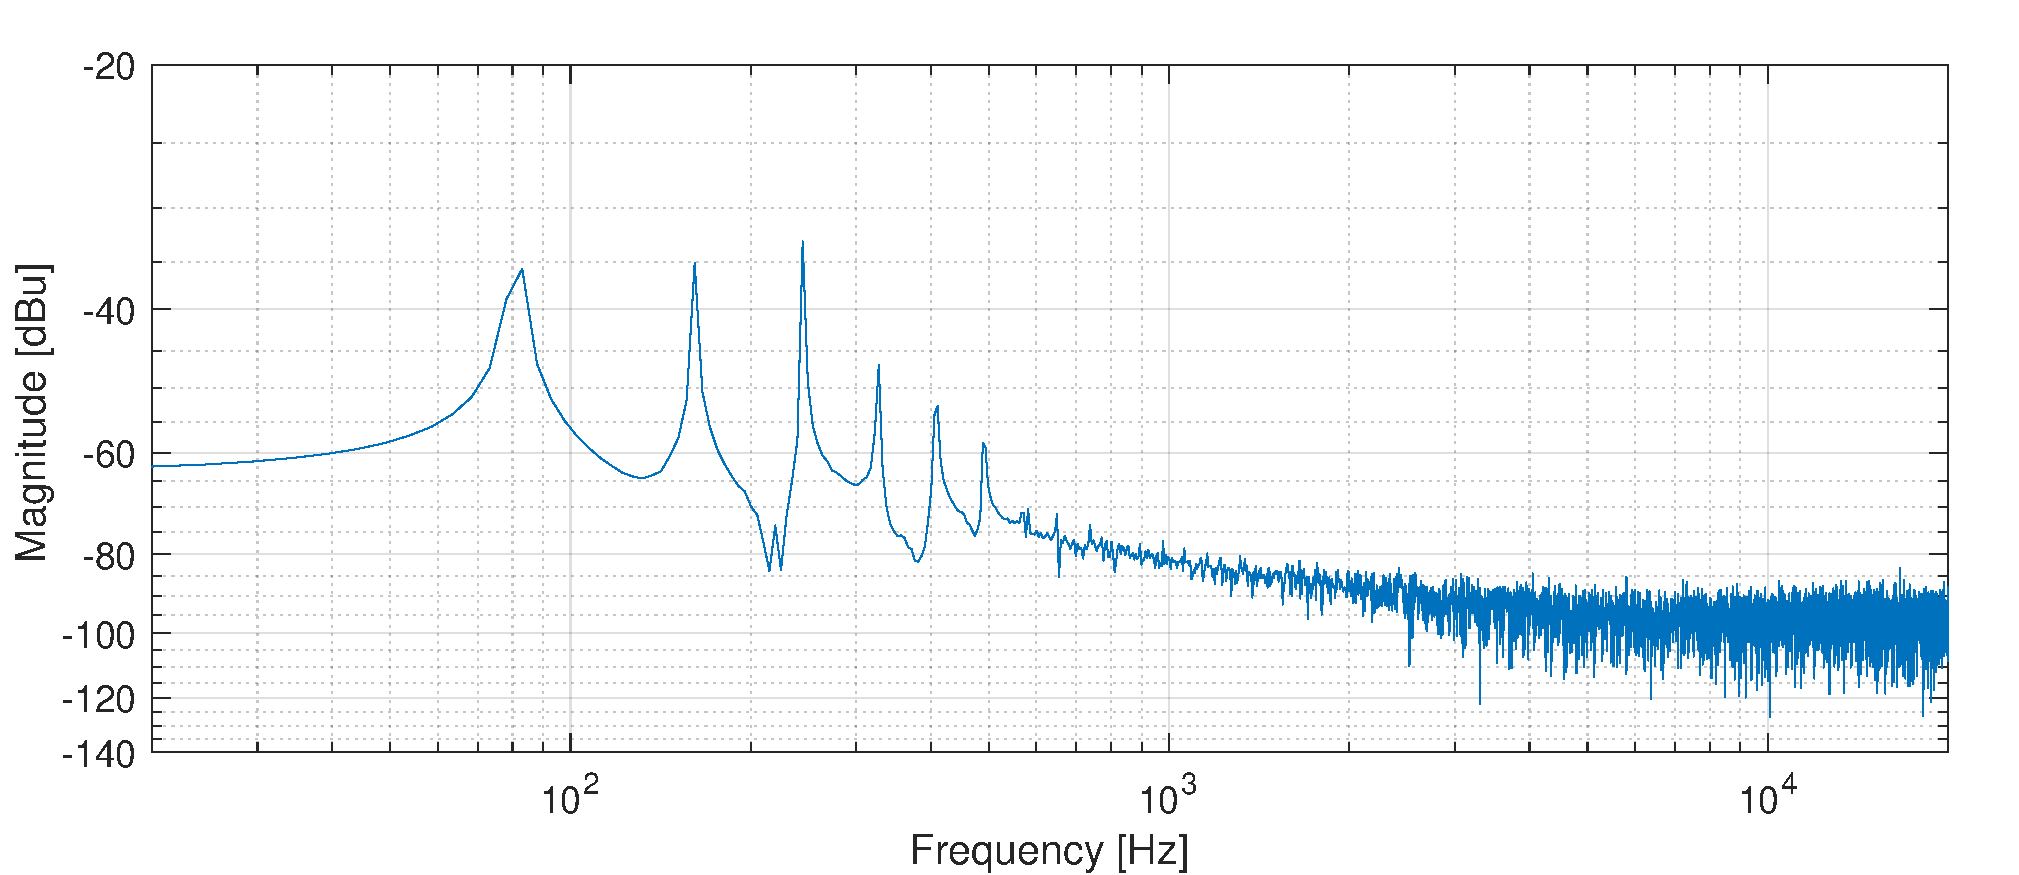
\includegraphics[width=1\textwidth]{guitar_low_E_neck.pdf}
		\caption{Measurement of the low E note on the neck pickup.}
		\label{fig:appendix:low_E_neck}
\end{figure}

On  \autoref{fig:appendix:low_E_neck} it is seen that the lowest significant frequency is around \SI{80}{\hertz} and the highest significant frequency is around \SI{400}{\hertz}, when playing the low E note on the guitar, using the neck pickup.

\begin{figure}[htbp!]
	\centering
		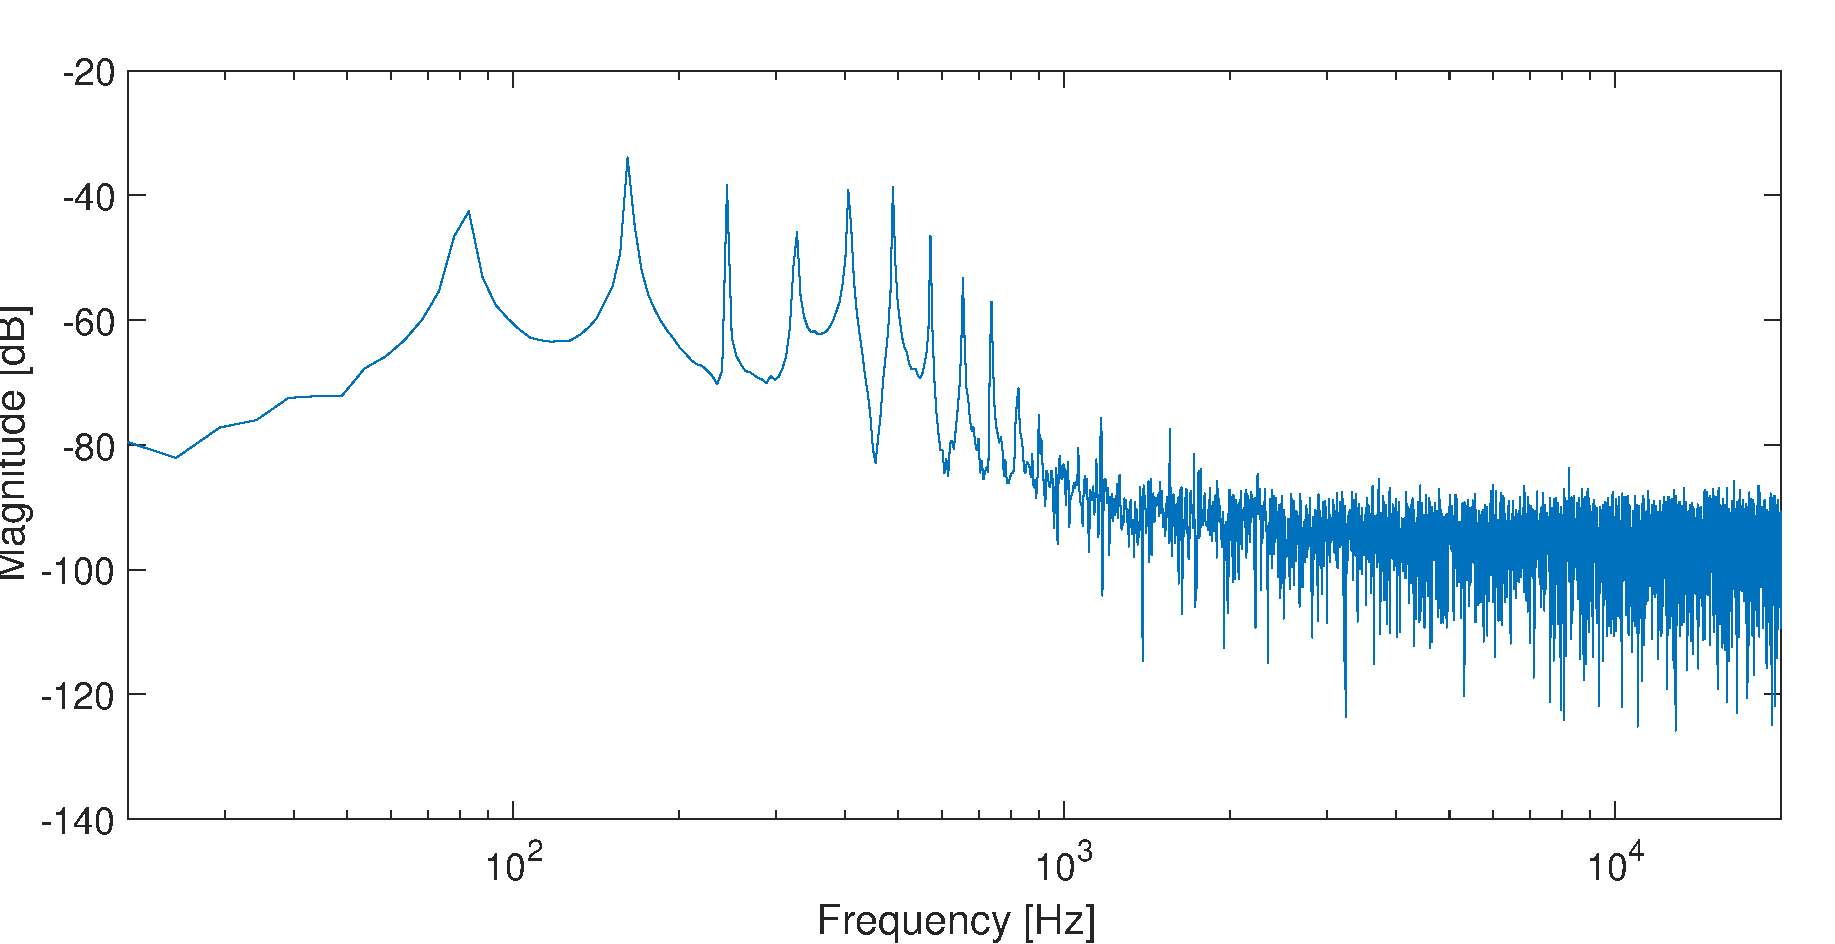
\includegraphics[width=1\textwidth]{guitar_low_E_bridge.pdf}
		\caption{Measurement of the low E note on the bridge pickup.}
		\label{fig:appendix:low_E_bridge}
\end{figure}

On  \autoref{fig:appendix:low_E_bridge} it is seen that the lowest significant frequency is around \SI{80}{\hertz} and the highest significant frequency is around \SI{730}{\hertz}, when playing the low E note on the guitar, using the bridge pickup.

\begin{figure}[htbp!]
	\centering
		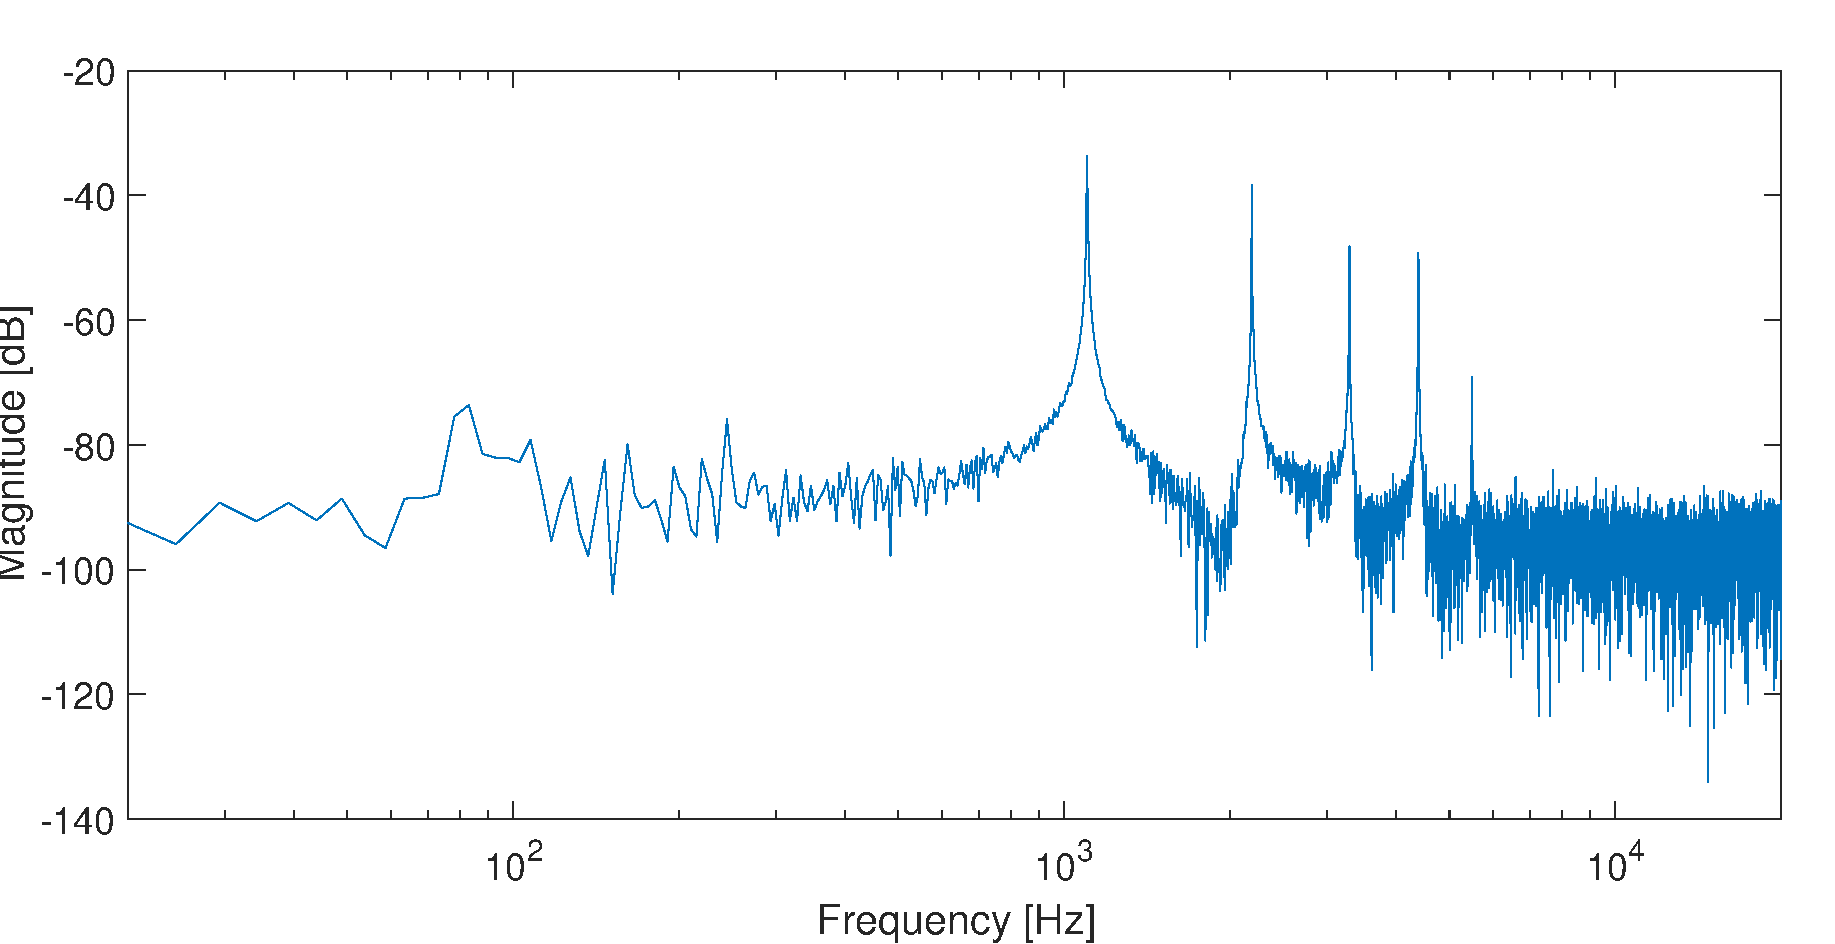
\includegraphics[width=1\textwidth]{guitar_high_Cis_neck.pdf}
		\caption{Measurement of the high C\# note on the neck pickup.}
		\label{fig:appendix:high_Cis_neck}
\end{figure}

On  \autoref{fig:appendix:high_Cis_neck} it is seen that the lowest significant frequency is around \SI{1100}{\hertz} and the highest significant frequency is around \SI{4400}{\hertz}, when playing the high C\# note on the guitar, using the neck pickup.

\begin{figure}[htbp!]
	\centering
		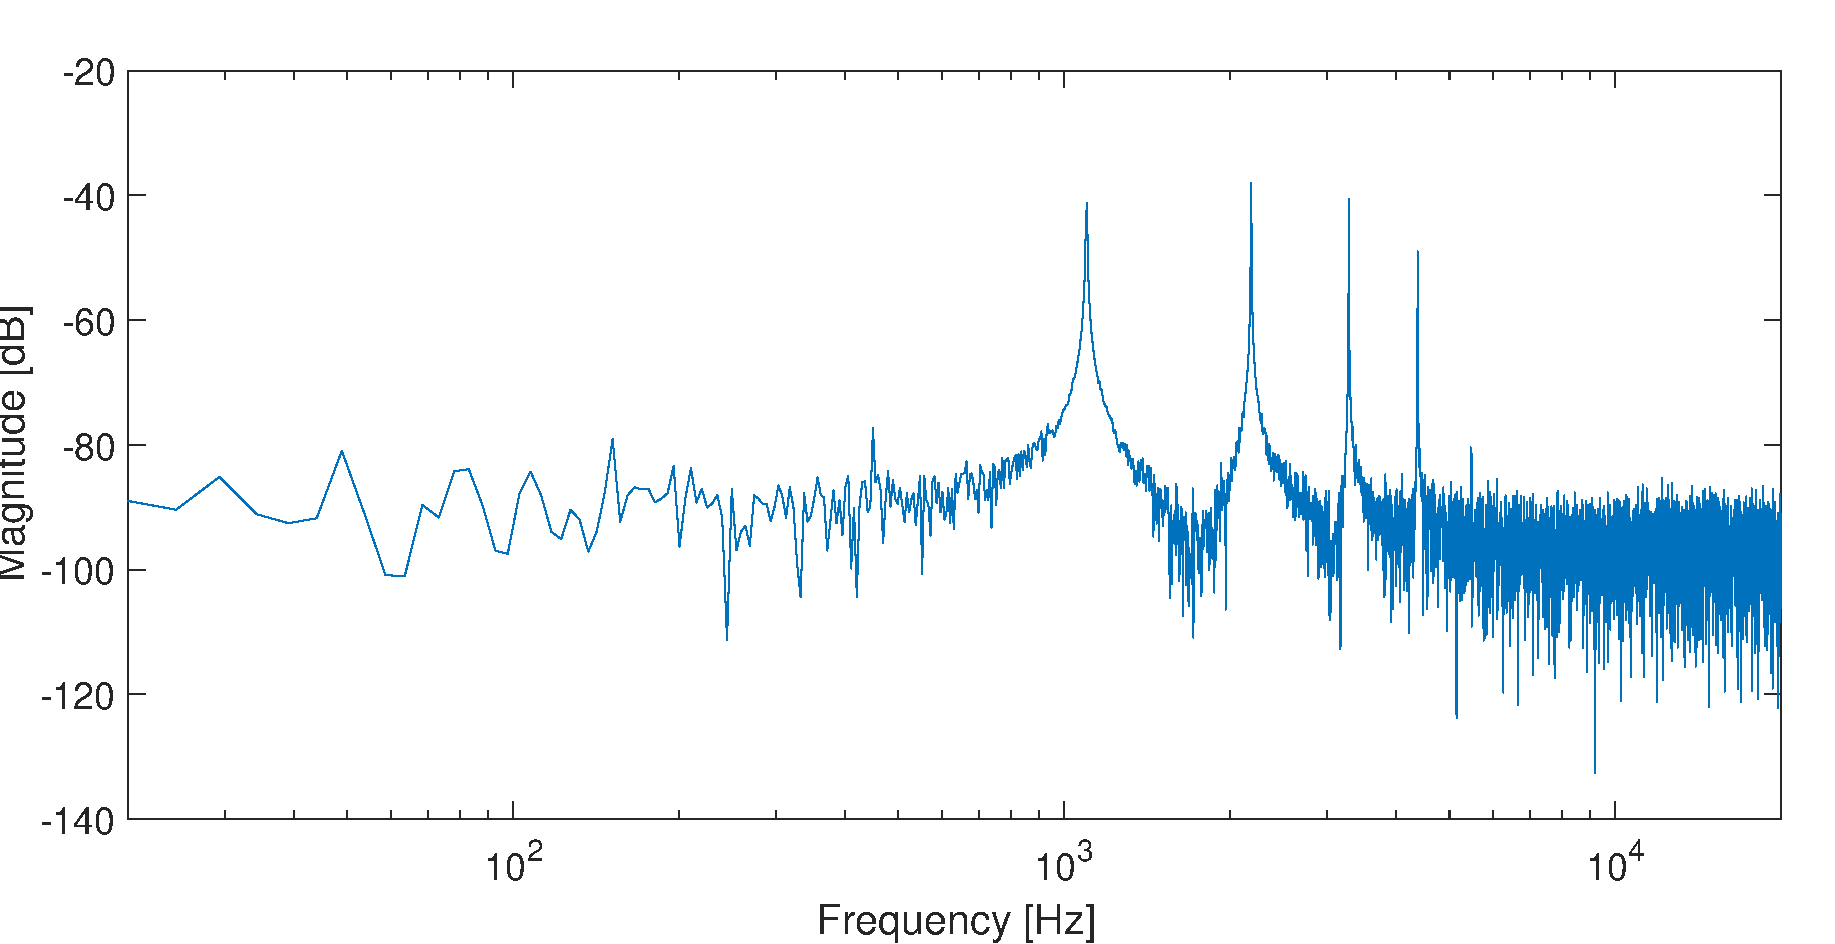
\includegraphics[width=1\textwidth]{guitar_high_Cis_bridge.pdf}
		\caption{Measurement of the high C\# note on the bridge pickup.}
		\label{fig:appendix:high_Cis_bridge}
\end{figure}

On  \autoref{fig:appendix:high_Cis_bridge} it is seen that the lowest significant frequency is around \SI{1100}{\hertz} and the highest significant frequency is around \SI{4400}{\hertz}, when playing the high C\# note on the guitar, using the bridge pickup. 

\begin{figure}[htbp!]
	\centering
		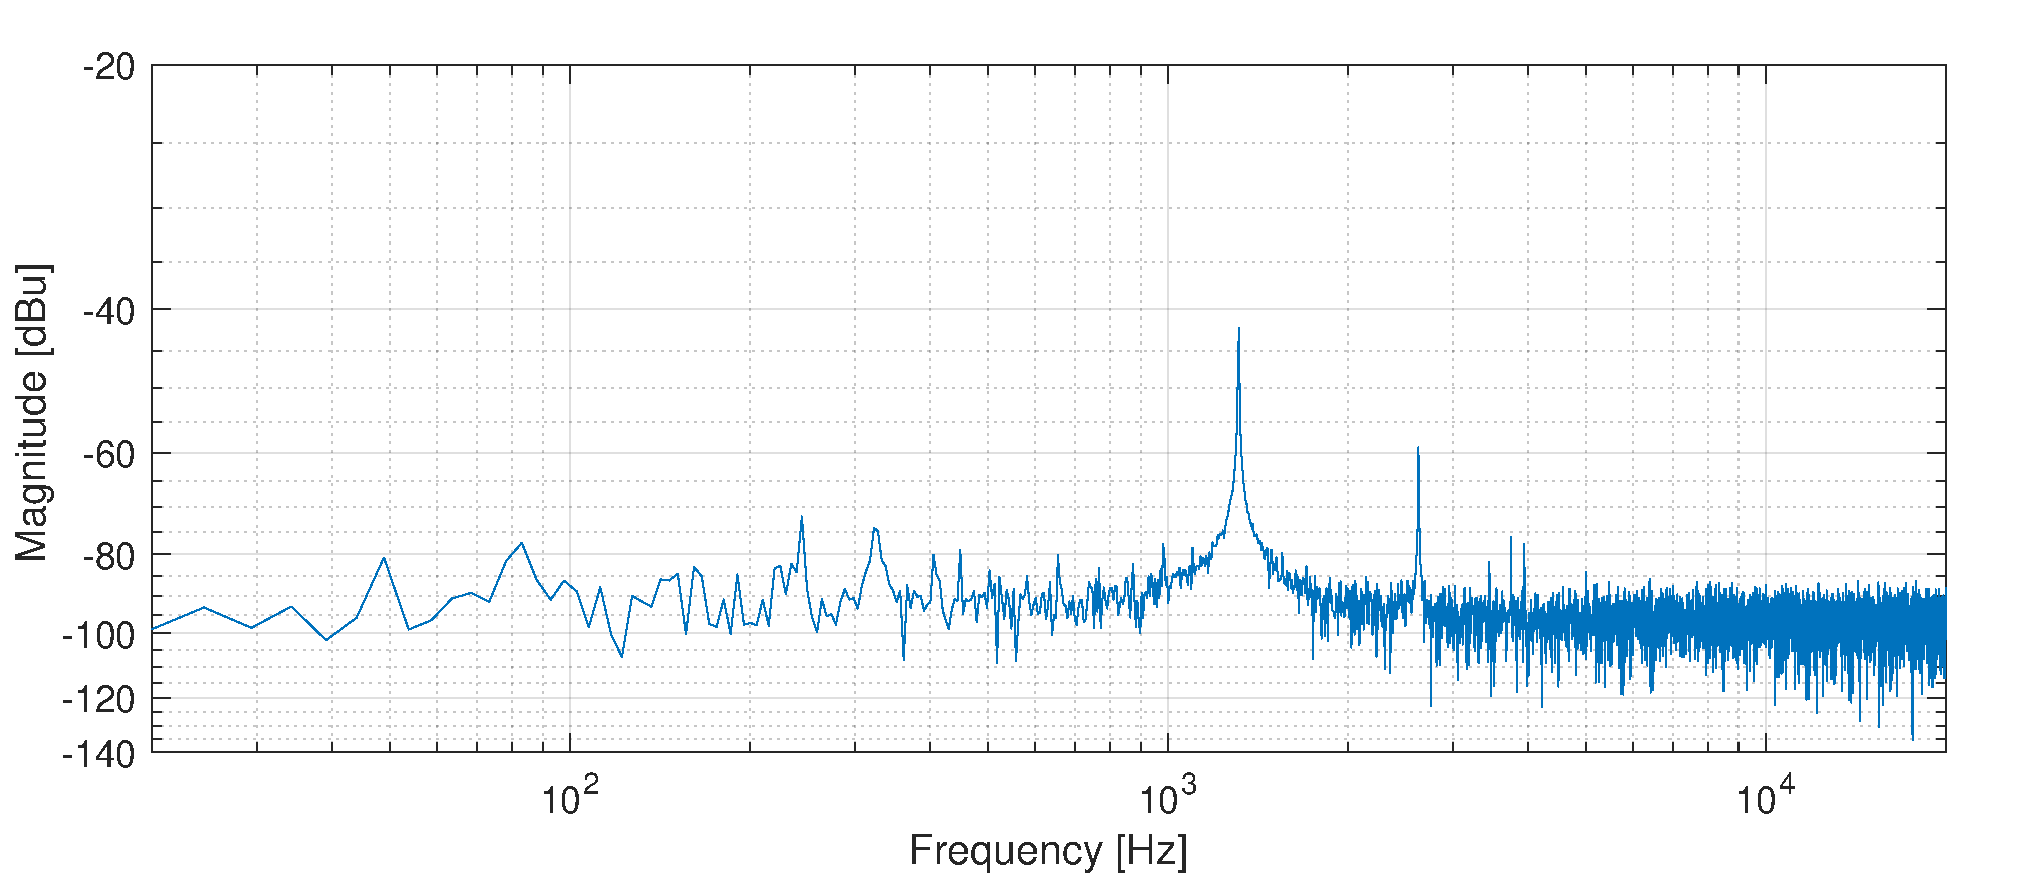
\includegraphics[width=1\textwidth]{guitar_high_E_flasholet_bridge.pdf}
		\caption{Measurement of the high E note, played as flasholet, on the bridge pickup.}
		\label{fig:appendix:high_E_bridge_flasholet}
\end{figure}

On  \autoref{fig:appendix:high_E_bridge_flasholet} it is seen that the lowest significant frequency is around \SI{1300}{\hertz} and the highest significant frequency is around \SI{2600}{\hertz}, when playing the high E note on the guitar as flasholet, using the bridge pickup. 

\caption{Setup for measuring frequency area on a guitar.}
		\label{fig:appendix:guitar_freq}
\end{figure}

\section*{Test procedure}
To the frequency area on a guitar, the following steps are made:
\begin{enumerate}
\item The materials are set up as in \autoref{fig:appendix:guitar_freq}.
\item Digilent Waveforms 2015 is set as a spectrum analyser. 
\item The guitar is set to use the neck pickup and the volume control and the tone control are turned all the way up.
\item The highest and the lowest tone on the guitar are played, measured by the oscilloscope and analysed in Digilent Waveforms 2015.
\item The guitar is set to use the bridge pickup and step 4 is repeated. 
\item The data is plotted in MATLAB.
\end{enumerate}

\section*{Results}

\begin{figure}[htbp!]
	\centering
		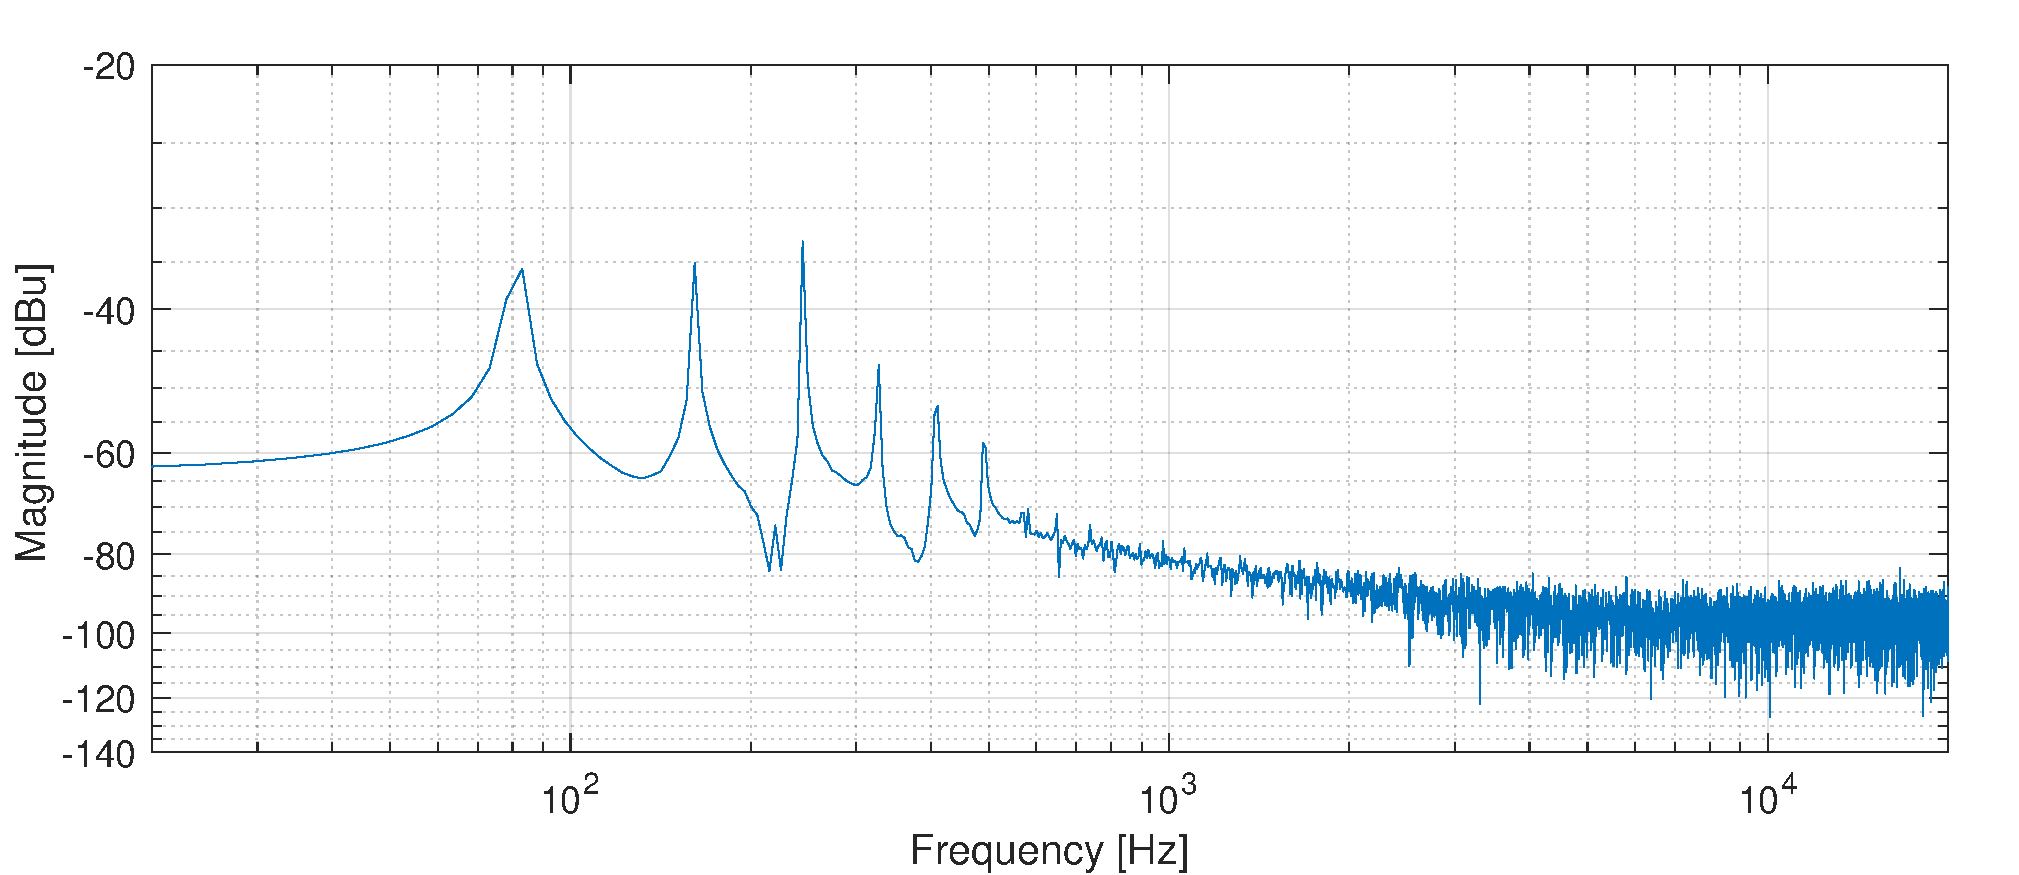
\includegraphics[width=1\textwidth]{guitar_low_E_neck.pdf}
		\caption{Measurement of the low E note on the neck pickup.}
		\label{fig:appendix:low_E_neck}
\end{figure}

On  \autoref{fig:appendix:low_E_neck} it is seen that the lowest significant frequency is around \SI{80}{\hertz} and the highest significant frequency is around \SI{400}{\hertz}, when playing the low E note on the guitar, using the neck pickup.

\begin{figure}[htbp!]
	\centering
		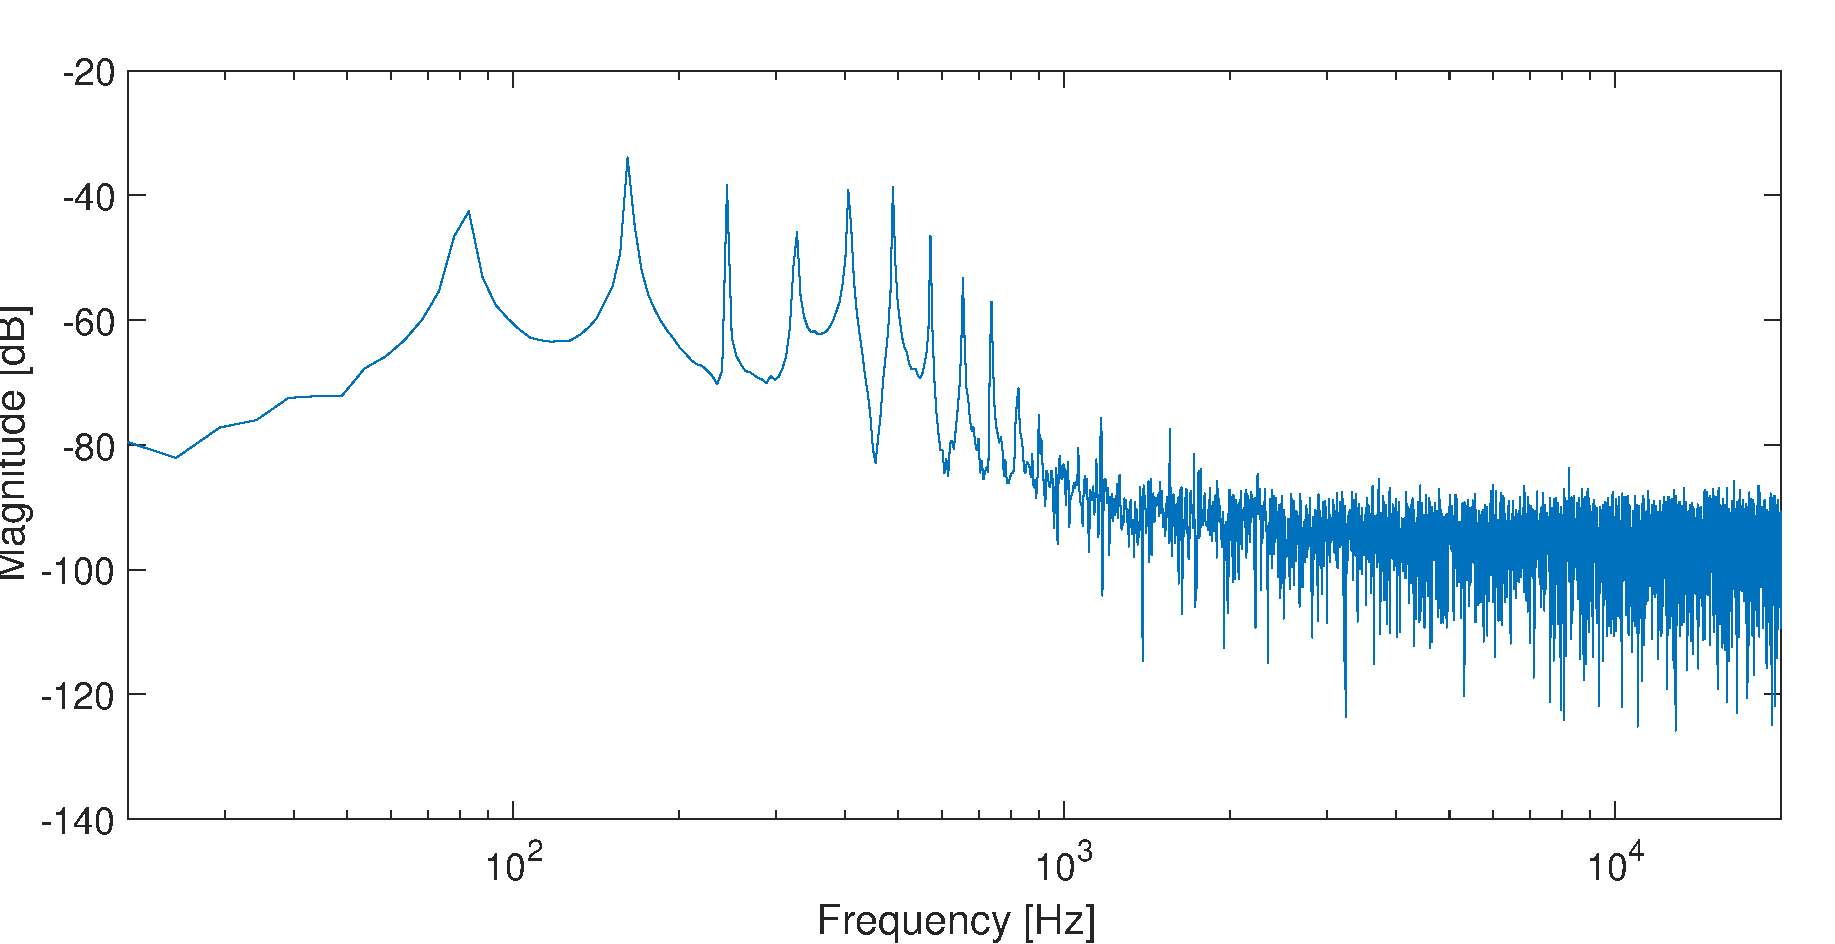
\includegraphics[width=1\textwidth]{guitar_low_E_bridge.pdf}
		\caption{Measurement of the low E note on the bridge pickup.}
		\label{fig:appendix:low_E_bridge}
\end{figure}

On  \autoref{fig:appendix:low_E_bridge} it is seen that the lowest significant frequency is around \SI{80}{\hertz} and the highest significant frequency is around \SI{730}{\hertz}, when playing the low E note on the guitar, using the bridge pickup.

\begin{figure}[htbp!]
	\centering
		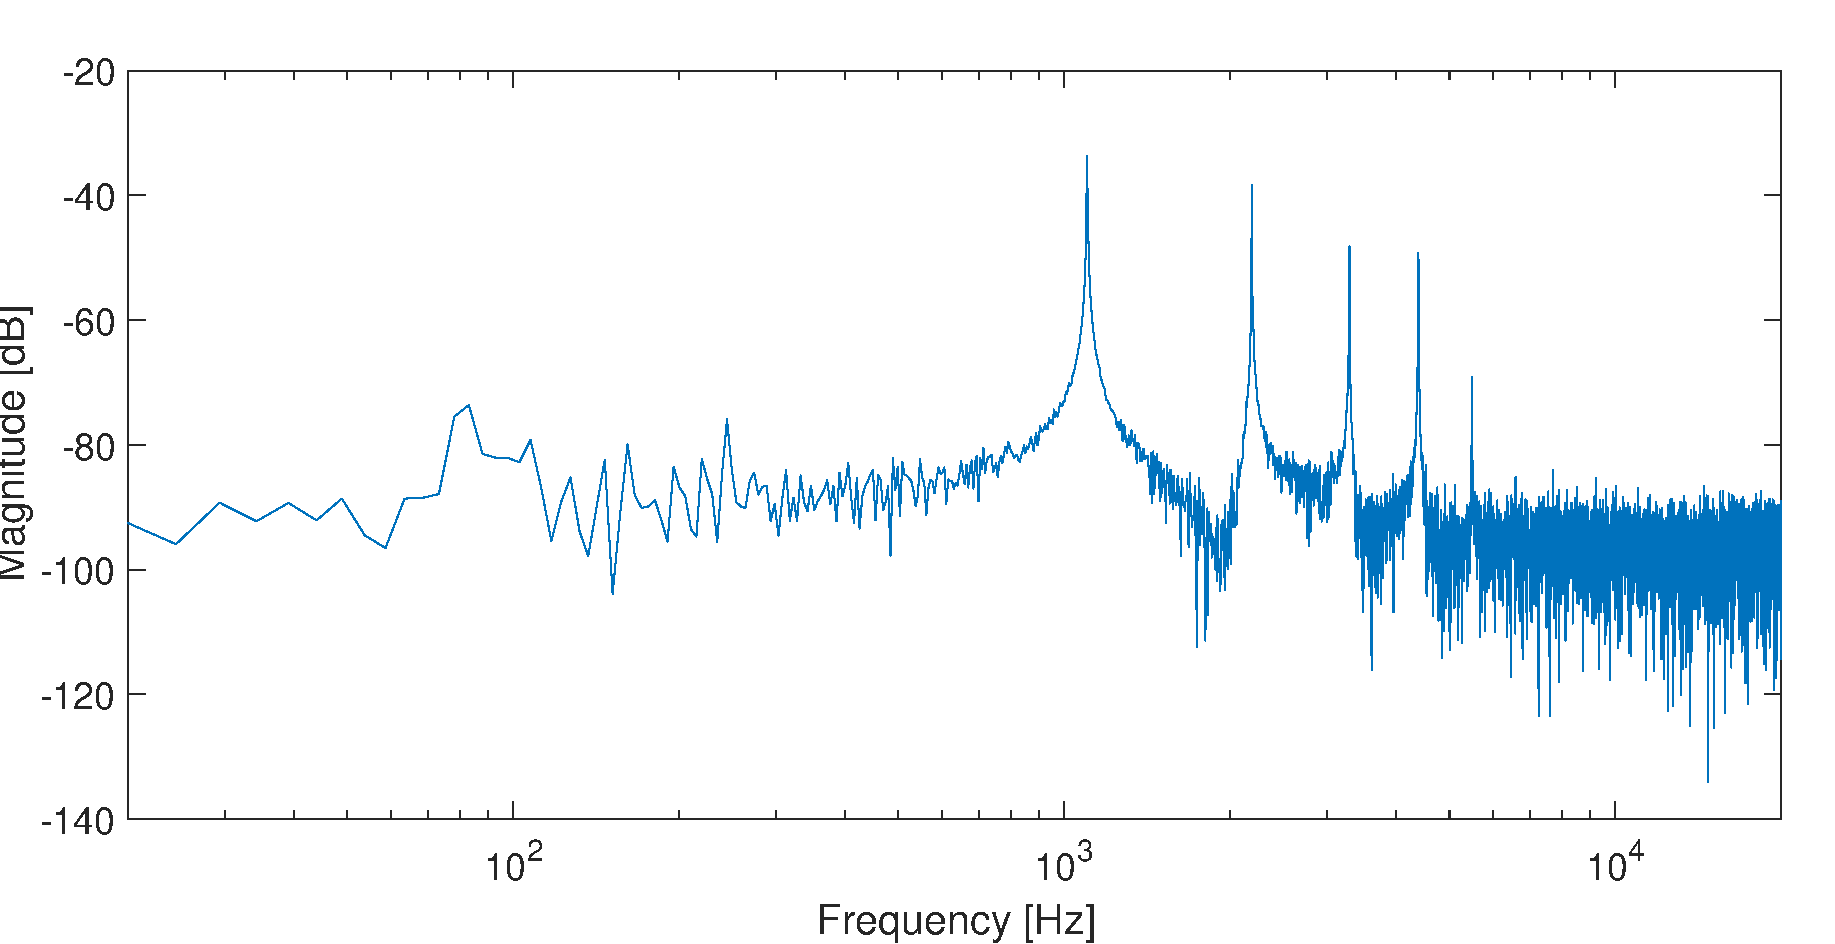
\includegraphics[width=1\textwidth]{guitar_high_Cis_neck.pdf}
		\caption{Measurement of the high C\# note on the neck pickup.}
		\label{fig:appendix:high_Cis_neck}
\end{figure}

On  \autoref{fig:appendix:high_Cis_neck} it is seen that the lowest significant frequency is around \SI{1100}{\hertz} and the highest significant frequency is around \SI{4400}{\hertz}, when playing the high C\# note on the guitar, using the neck pickup.

\begin{figure}[htbp!]
	\centering
		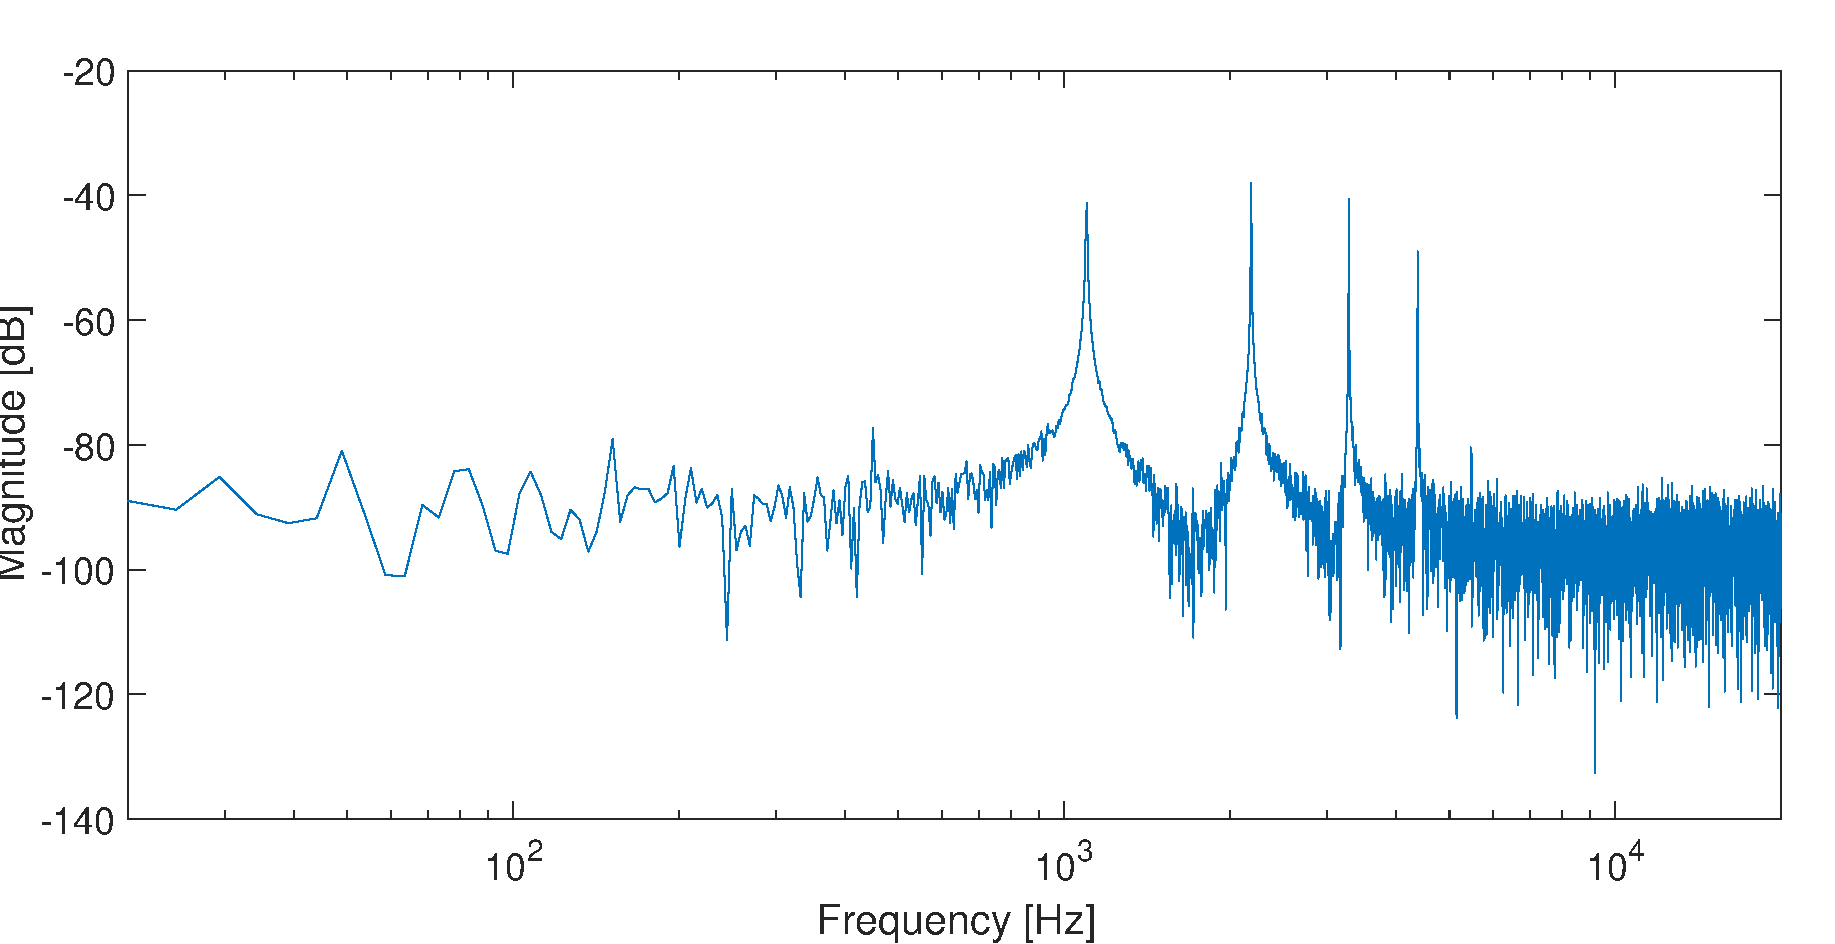
\includegraphics[width=1\textwidth]{guitar_high_Cis_bridge.pdf}
		\caption{Measurement of the high C\# note on the bridge pickup.}
		\label{fig:appendix:high_Cis_bridge}
\end{figure}

On  \autoref{fig:appendix:high_Cis_bridge} it is seen that the lowest significant frequency is around \SI{1100}{\hertz} and the highest significant frequency is around \SI{4400}{\hertz}, when playing the high C\# note on the guitar, using the bridge pickup. 

\begin{figure}[htbp!]
	\centering
		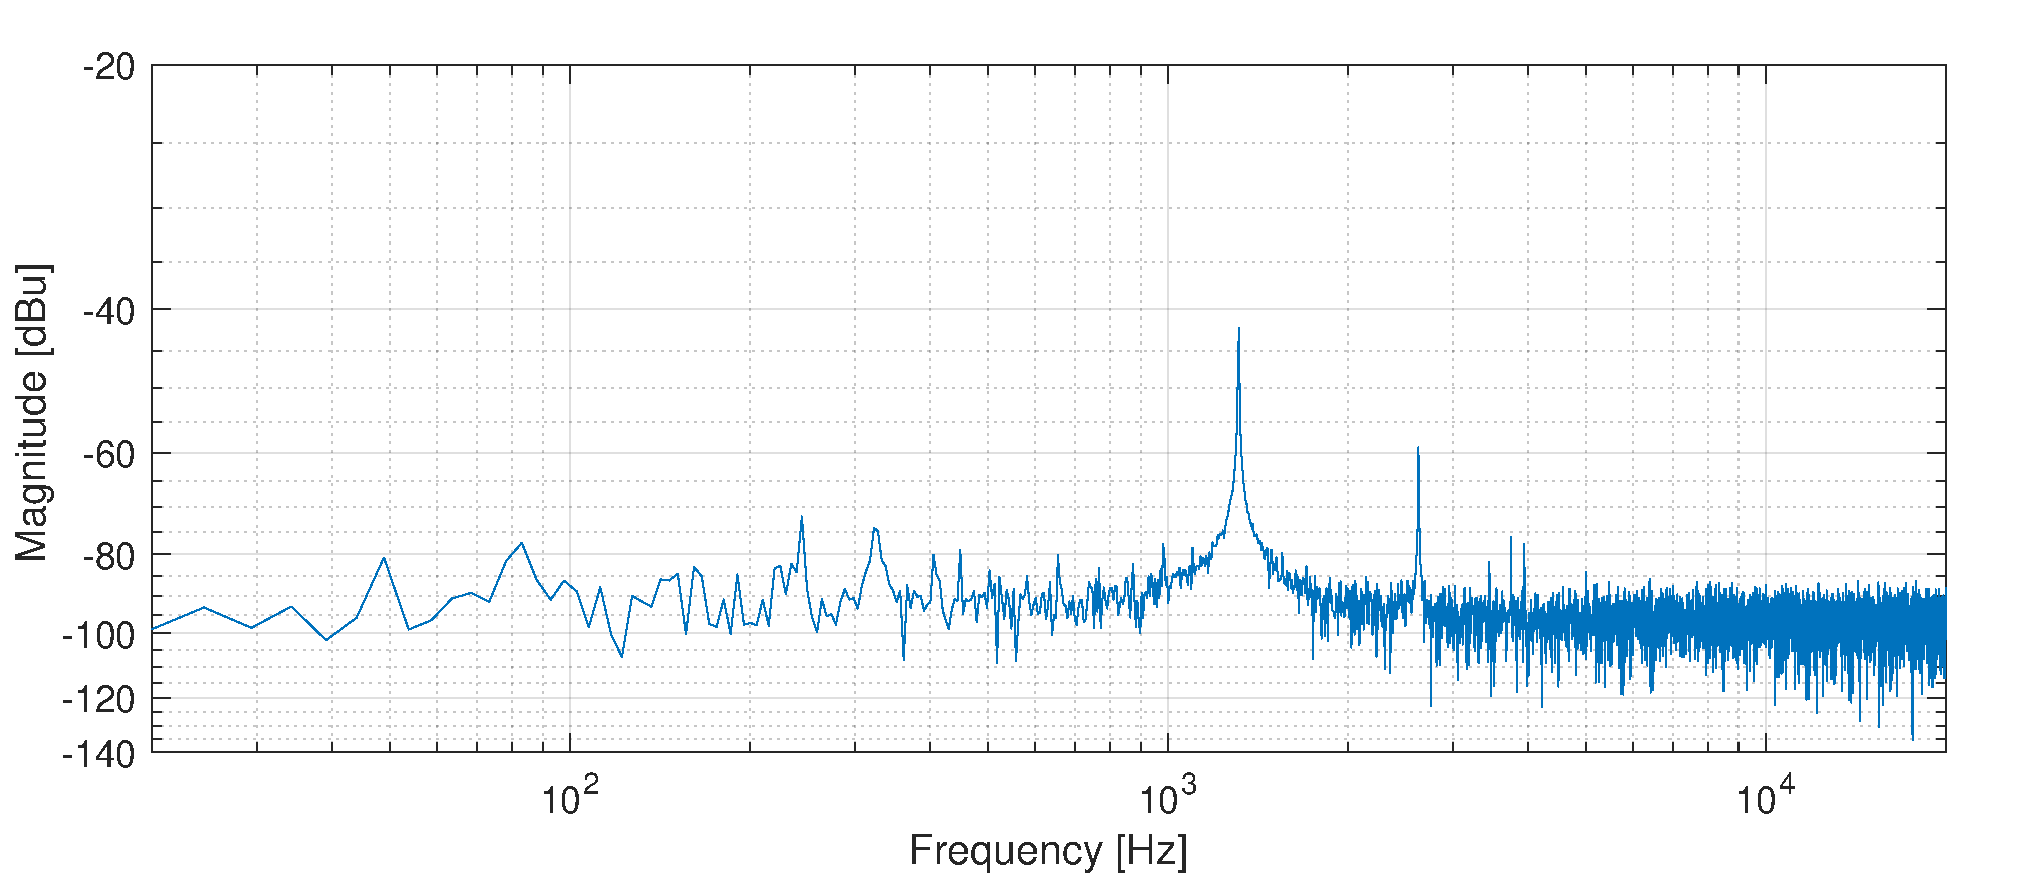
\includegraphics[width=1\textwidth]{guitar_high_E_flasholet_bridge.pdf}
		\caption{Measurement of the high E note, played as flasholet, on the bridge pickup.}
		\label{fig:appendix:high_E_bridge_flasholet}
\end{figure}

On  \autoref{fig:appendix:high_E_bridge_flasholet} it is seen that the lowest significant frequency is around \SI{1300}{\hertz} and the highest significant frequency is around \SI{2600}{\hertz}, when playing the high E note on the guitar as flasholet, using the bridge pickup. 

\caption{Setup for measuring frequency area on a guitar.}
		\label{fig:appendix:guitar_freq}
\end{figure}

\section*{Test procedure}
To the frequency area on a guitar, the following steps are made:
\begin{enumerate}
\item The materials are set up as in \autoref{fig:appendix:guitar_freq}.
\item Digilent Waveforms 2015 is set as a spectrum analyser. 
\item The guitar is set to use the neck pickup and the volume control and the tone control are turned all the way up.
\item The highest and the lowest tone on the guitar are played, measured by the oscilloscope and analysed in Digilent Waveforms 2015.
\item The guitar is set to use the bridge pickup and step 4 is repeated. 
\item The data is plotted in MATLAB.
\end{enumerate}

\section*{Results}

\begin{figure}[htbp!]
	\centering
		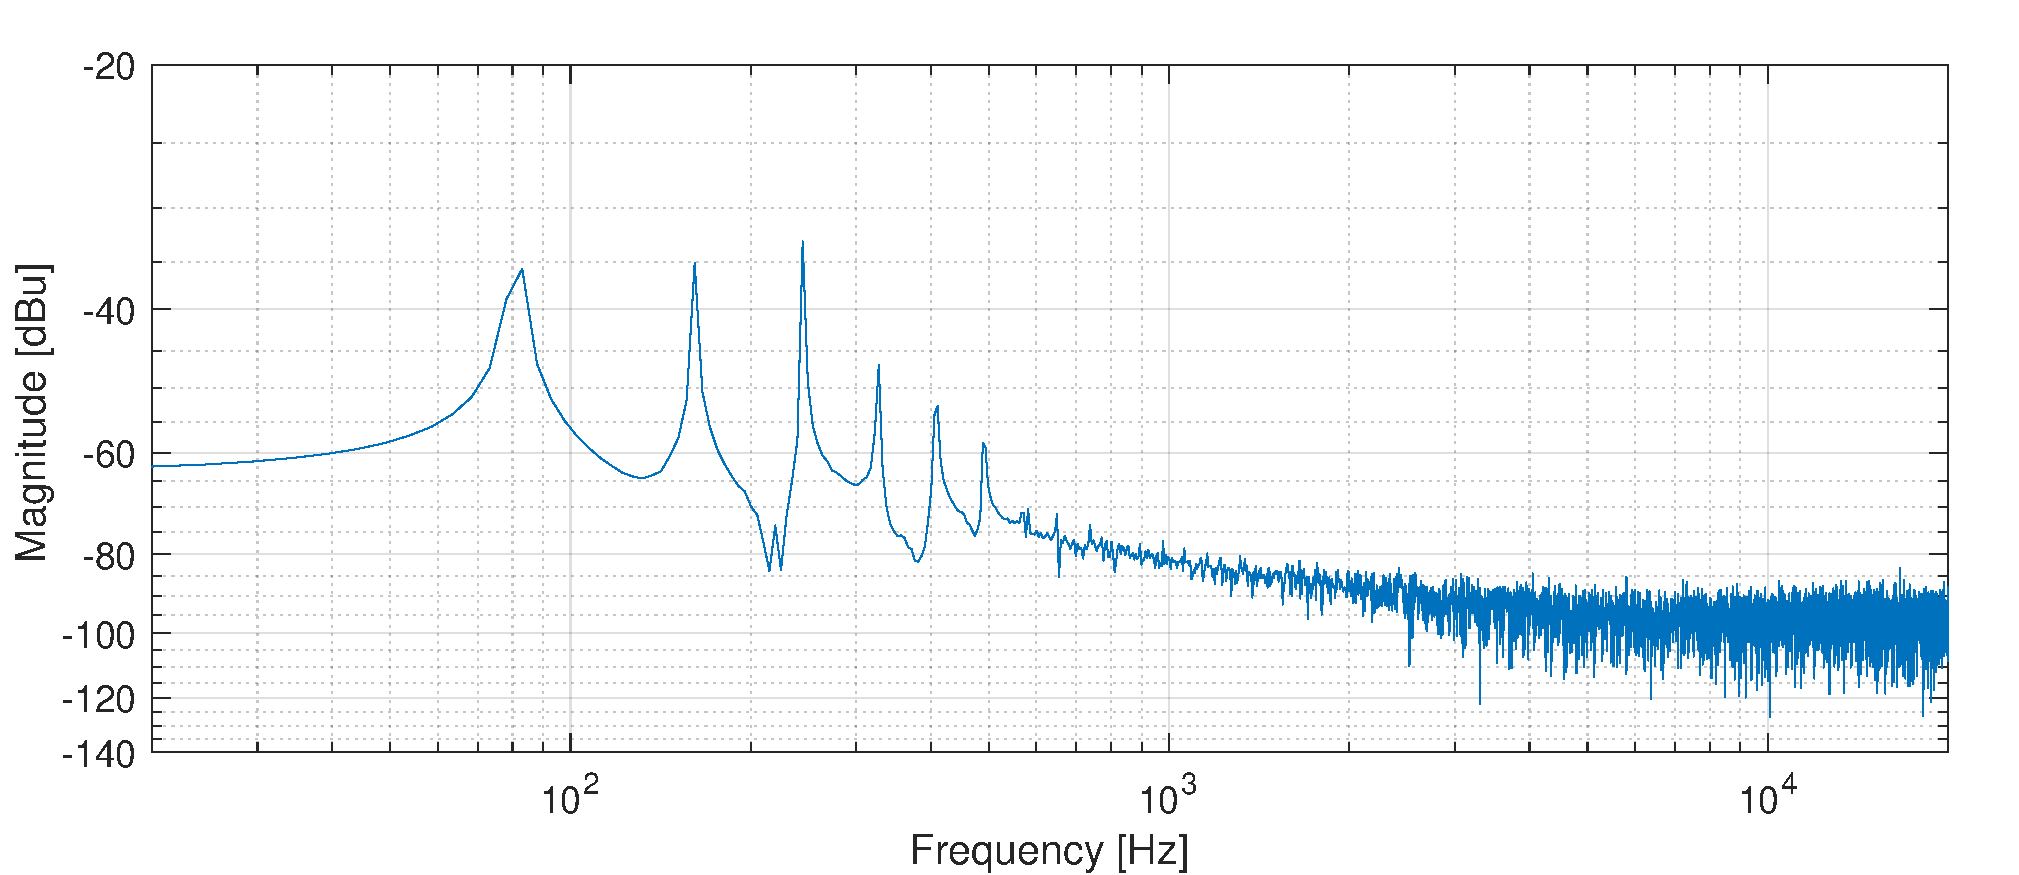
\includegraphics[width=1\textwidth]{guitar_low_E_neck.pdf}
		\caption{Measurement of the low E note on the neck pickup.}
		\label{fig:appendix:low_E_neck}
\end{figure}

On  \autoref{fig:appendix:low_E_neck} it is seen that the lowest significant frequency is around \SI{80}{\hertz} and the highest significant frequency is around \SI{400}{\hertz}, when playing the low E note on the guitar, using the neck pickup.

\begin{figure}[htbp!]
	\centering
		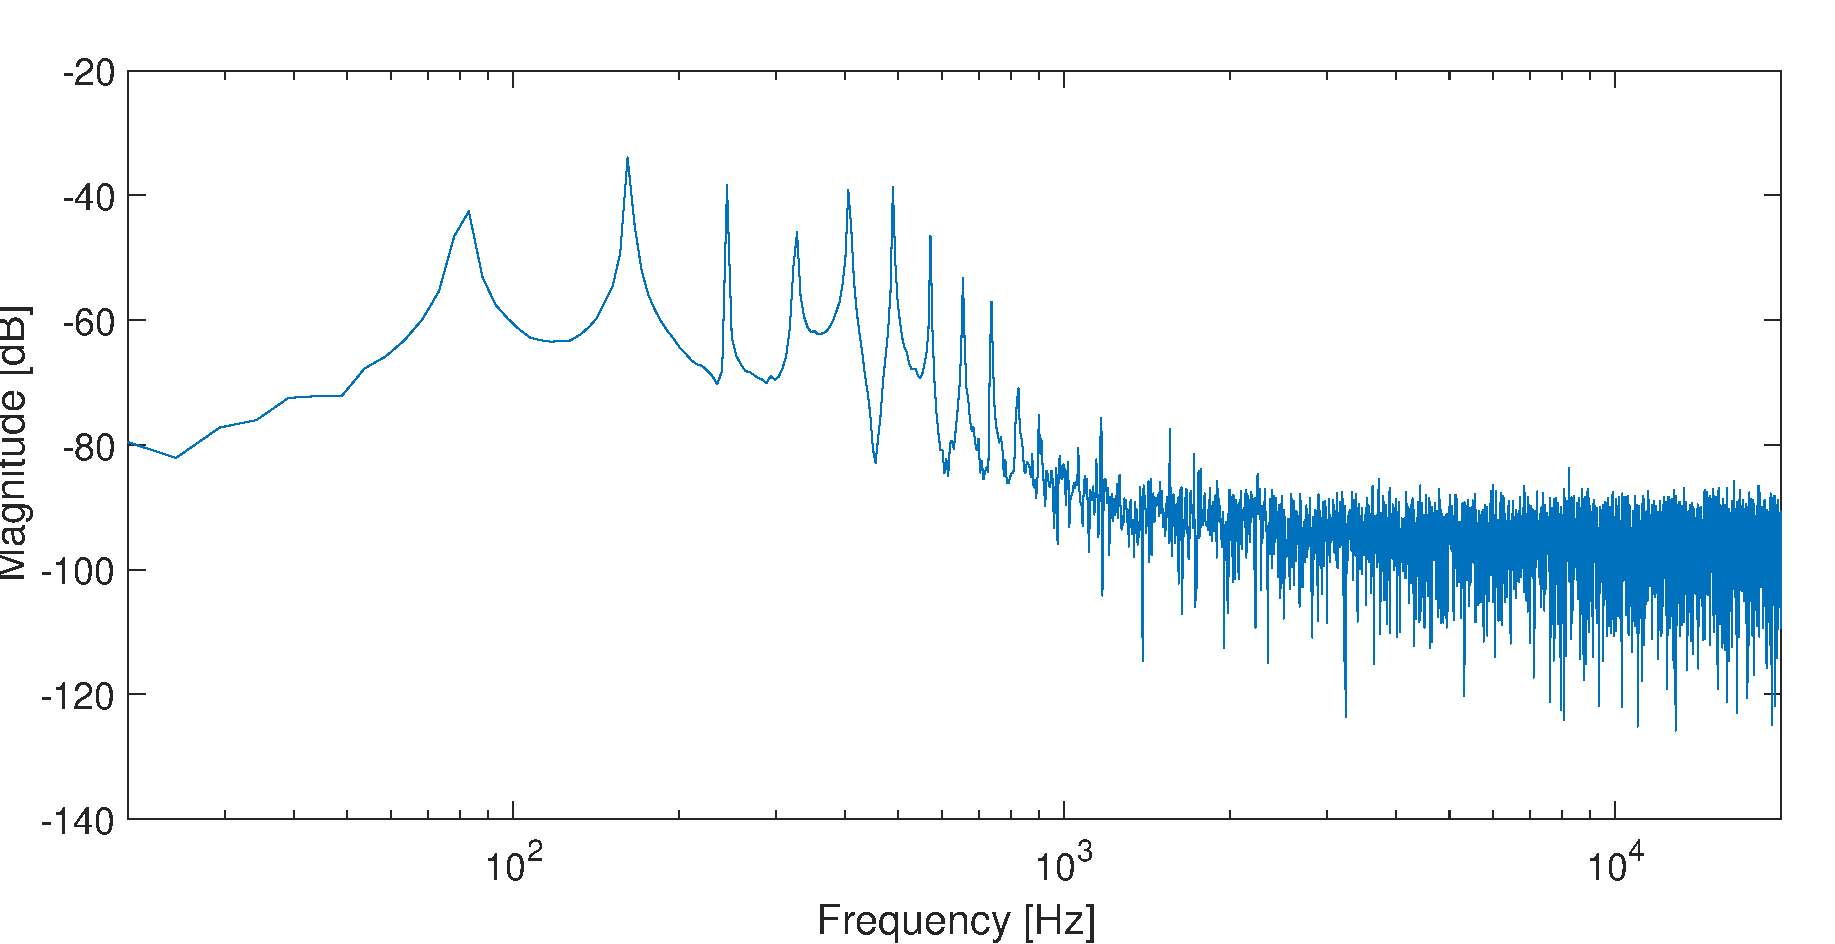
\includegraphics[width=1\textwidth]{guitar_low_E_bridge.pdf}
		\caption{Measurement of the low E note on the bridge pickup.}
		\label{fig:appendix:low_E_bridge}
\end{figure}

On  \autoref{fig:appendix:low_E_bridge} it is seen that the lowest significant frequency is around \SI{80}{\hertz} and the highest significant frequency is around \SI{730}{\hertz}, when playing the low E note on the guitar, using the bridge pickup.

\begin{figure}[htbp!]
	\centering
		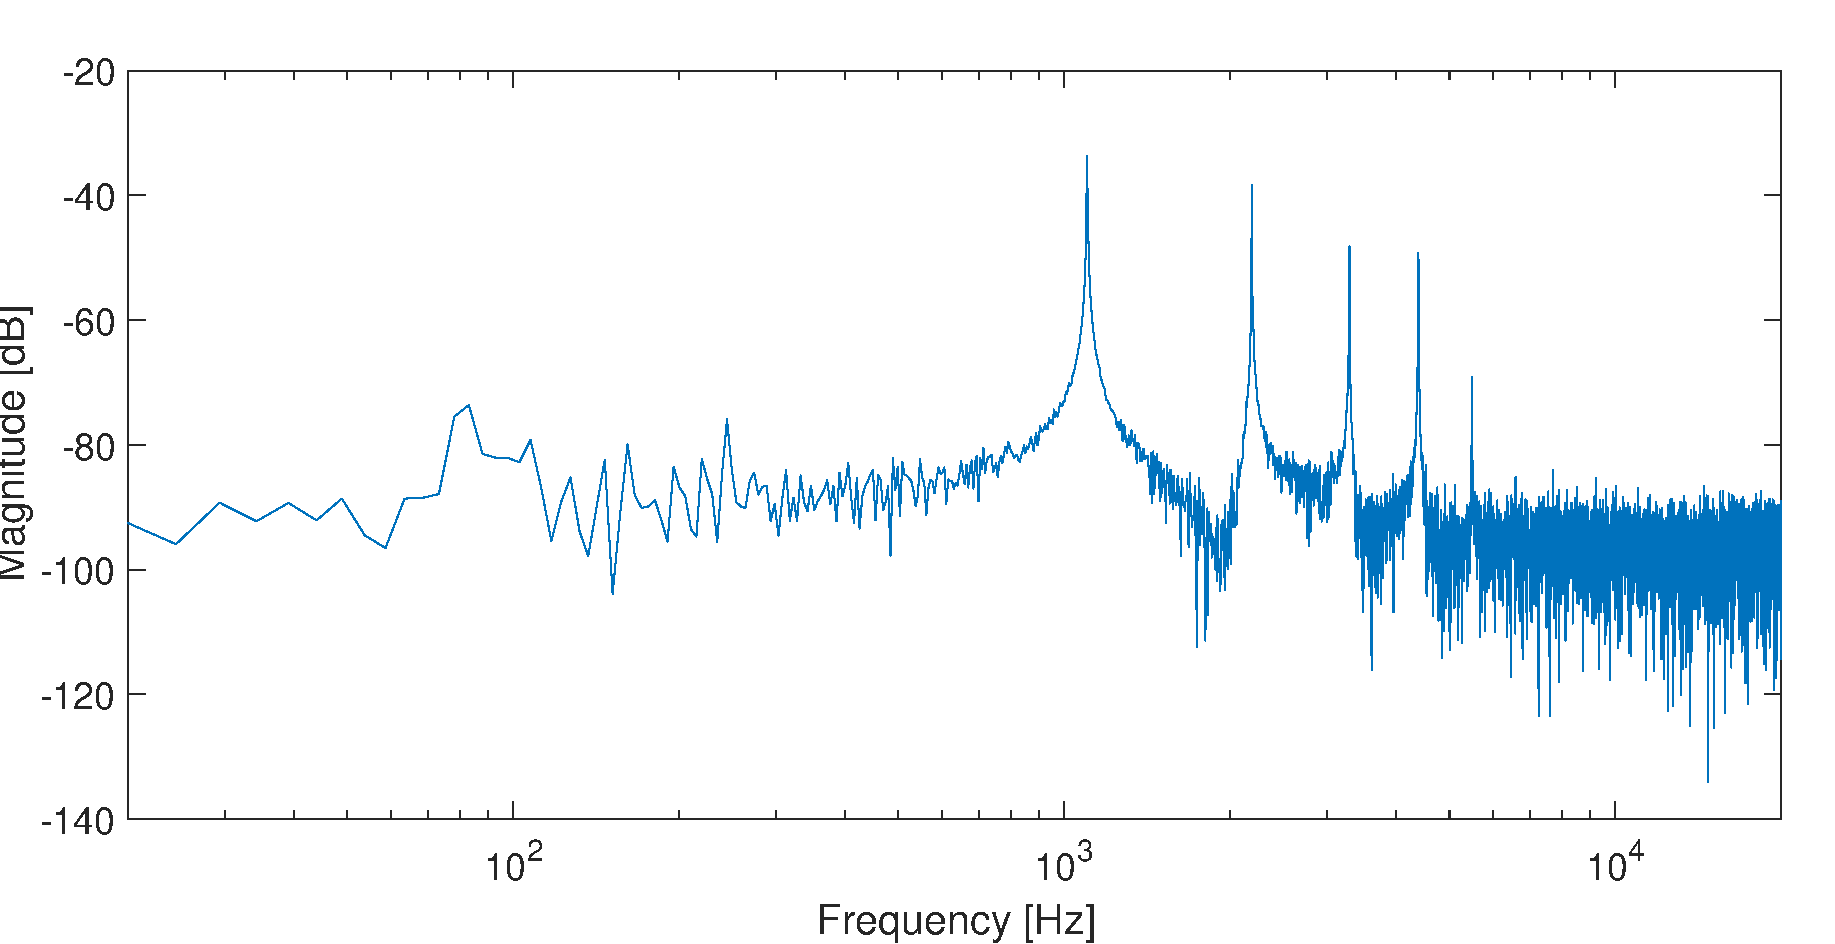
\includegraphics[width=1\textwidth]{guitar_high_Cis_neck.pdf}
		\caption{Measurement of the high C\# note on the neck pickup.}
		\label{fig:appendix:high_Cis_neck}
\end{figure}

On  \autoref{fig:appendix:high_Cis_neck} it is seen that the lowest significant frequency is around \SI{1100}{\hertz} and the highest significant frequency is around \SI{4400}{\hertz}, when playing the high C\# note on the guitar, using the neck pickup.

\begin{figure}[htbp!]
	\centering
		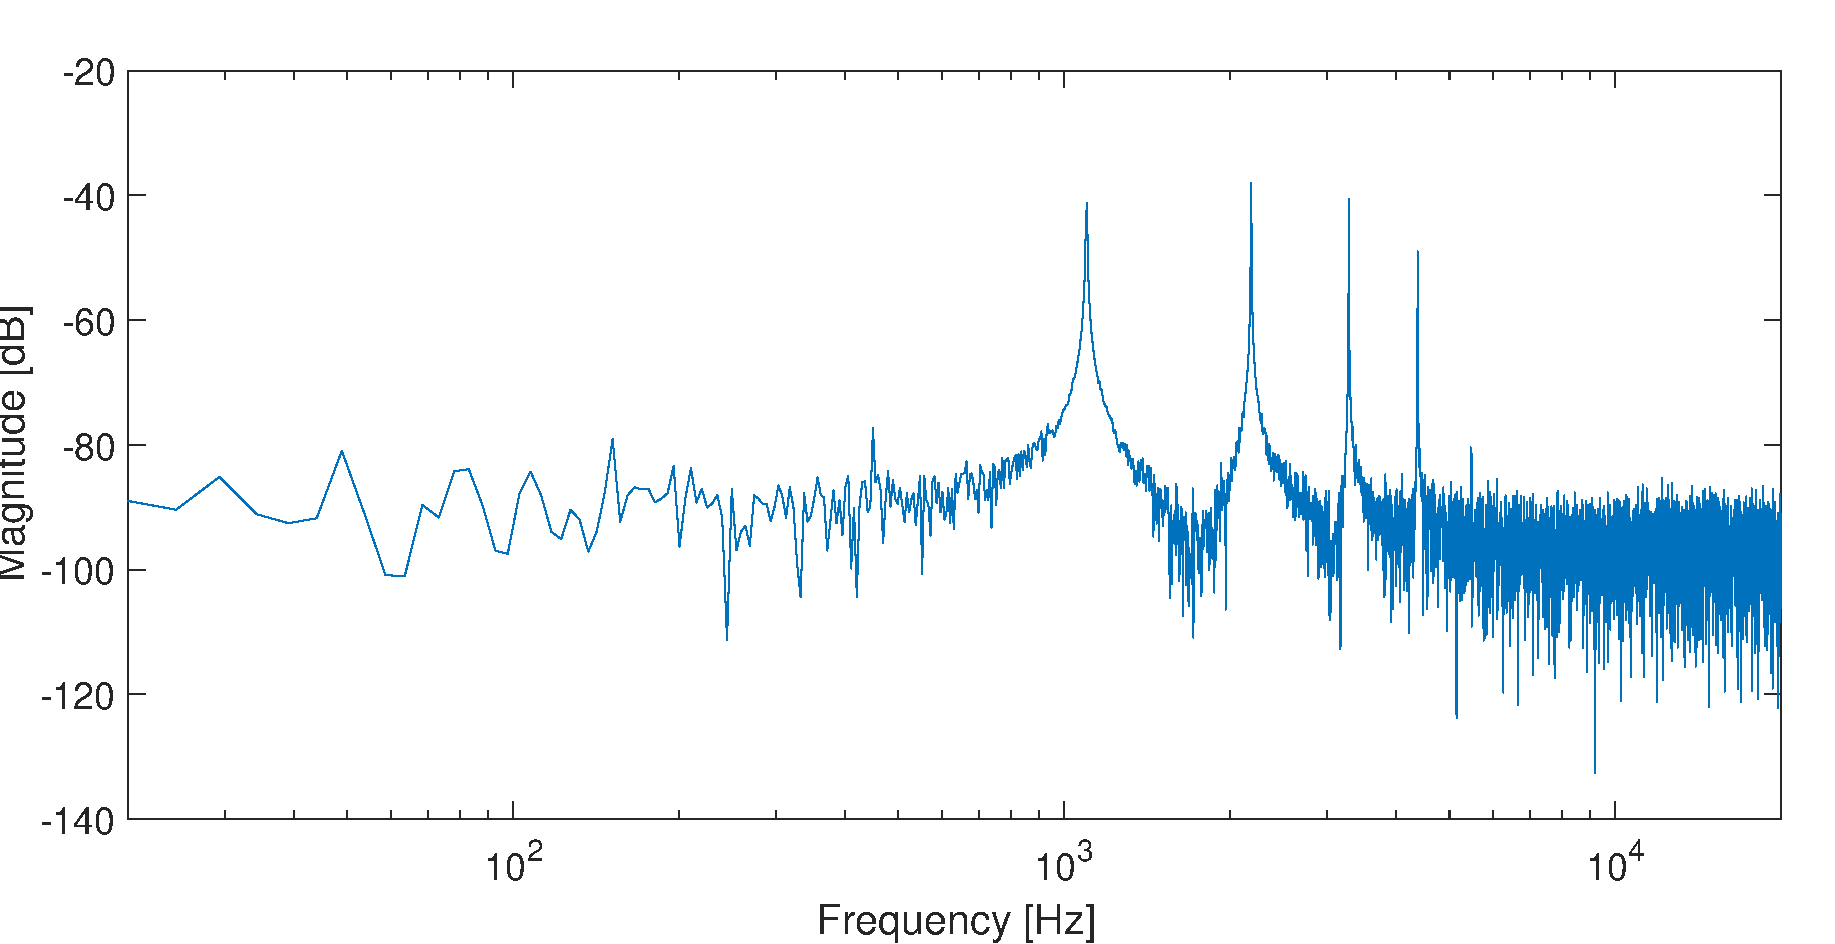
\includegraphics[width=1\textwidth]{guitar_high_Cis_bridge.pdf}
		\caption{Measurement of the high C\# note on the bridge pickup.}
		\label{fig:appendix:high_Cis_bridge}
\end{figure}

On  \autoref{fig:appendix:high_Cis_bridge} it is seen that the lowest significant frequency is around \SI{1100}{\hertz} and the highest significant frequency is around \SI{4400}{\hertz}, when playing the high C\# note on the guitar, using the bridge pickup. 

\begin{figure}[htbp!]
	\centering
		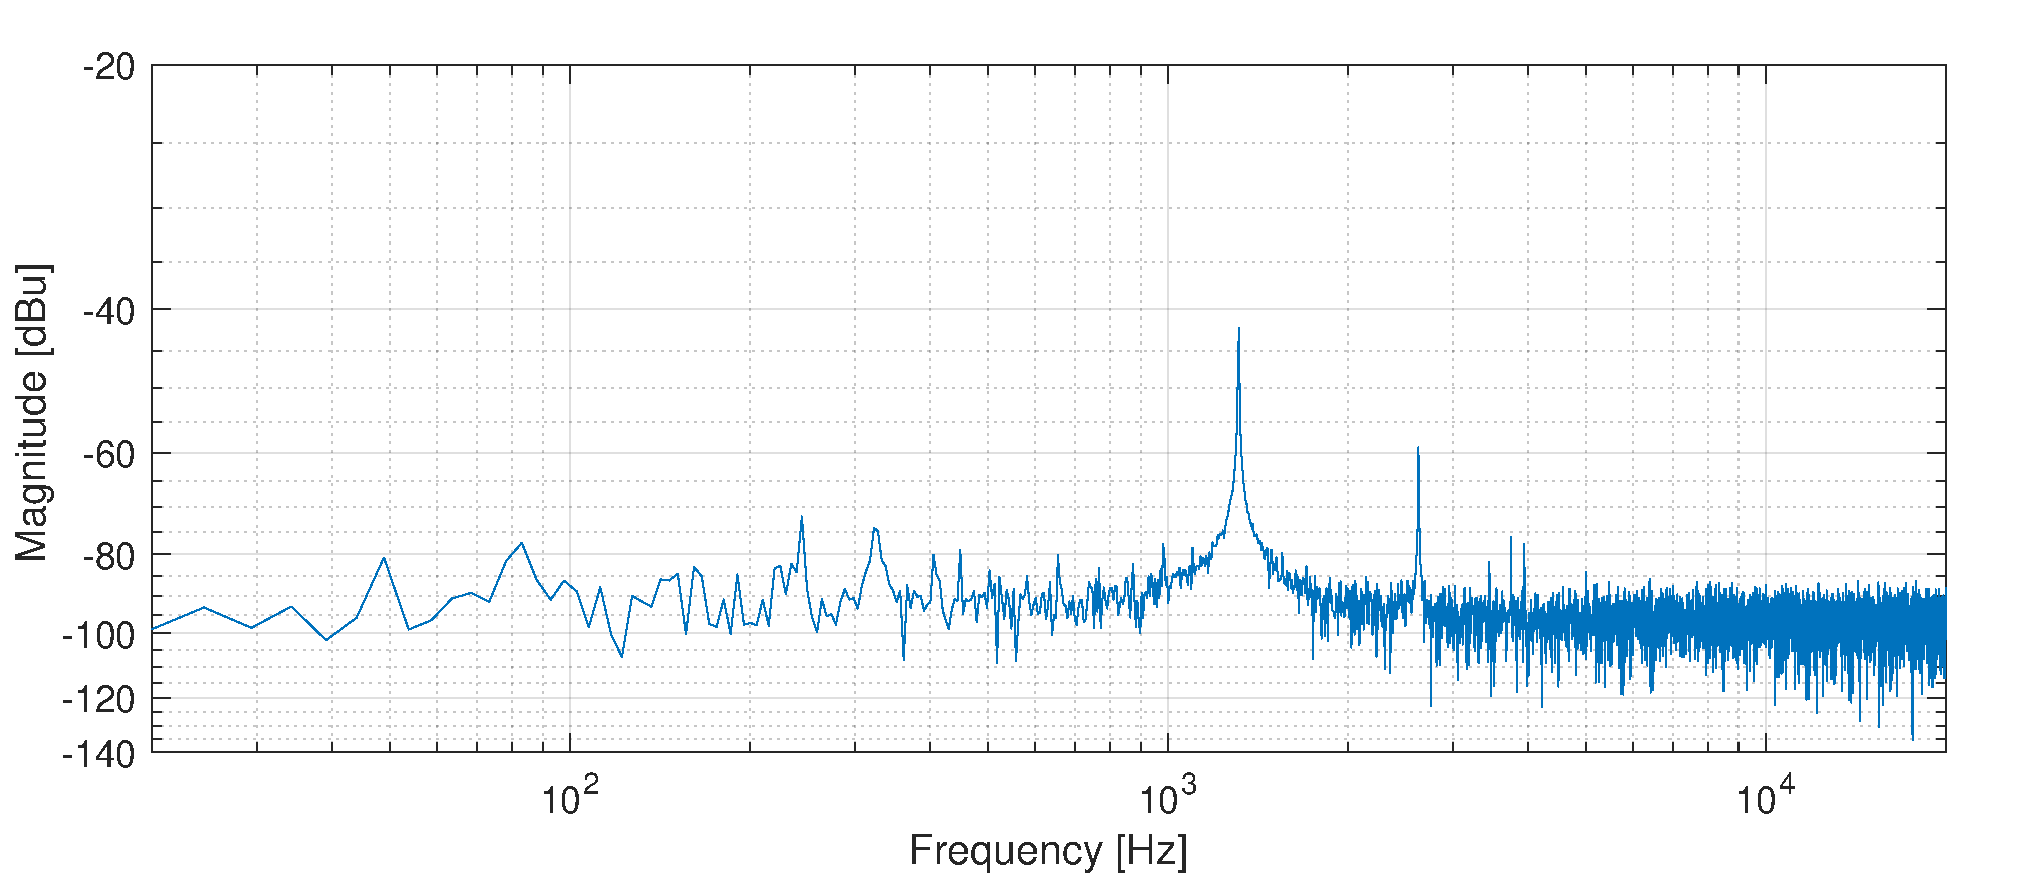
\includegraphics[width=1\textwidth]{guitar_high_E_flasholet_bridge.pdf}
		\caption{Measurement of the high E note, played as flasholet, on the bridge pickup.}
		\label{fig:appendix:high_E_bridge_flasholet}
\end{figure}

On  \autoref{fig:appendix:high_E_bridge_flasholet} it is seen that the lowest significant frequency is around \SI{1300}{\hertz} and the highest significant frequency is around \SI{2600}{\hertz}, when playing the high E note on the guitar as flasholet, using the bridge pickup. 

\caption{Setup for measuring frequency area on a guitar.}
		\label{fig:appendix:guitar_freq}
\end{figure}

\section*{Test procedure}
To the frequency area on a guitar, the following steps are made:
\begin{enumerate}
\item The materials are set up as in \autoref{fig:appendix:guitar_freq}.
\item Digilent Waveforms 2015 is set as a spectrum analyser. 
\item The guitar is set to use the neck pickup and the volume control and the tone control are turned all the way up.
\item The highest and the lowest tone on the guitar are played, measured by the oscilloscope and analysed in Digilent Waveforms 2015.
\item The guitar is set to use the bridge pickup and step 4 is repeated. 
\item The data is plotted in MATLAB.
\end{enumerate}

\section*{Results}

